\section{Our Structure}
\begin{figure}[!h]
    \centering
    \includegraphics[width=0.5\columnwidth]{./OurStructure.png}
    \caption{Adele's Structure}
    \label{fig:adele_structure}
\end{figure}

\subsection{Kinect Node: Gestures}
Gesture recognition can be performed by tracking the movements of the different parts of the body. Once a stable detection of the joints is made, following them is the starting point towards the gesture recognition. 

Using a tracking software, the stable detection was achieved using a median filter of 5 samples.  Extracting these features from the image allow the construction of small movements and/or complete gestures. From points representing joints it's straightforward to use vectors to represent parts of the body like arm and forearm. Relations between them, such as angles or distances perform a good way to detect movements independent from the camera's referential.  

Not only the dislocation of the joints positions but also features as velocities and accelerations are detected. This way small movements are recognize as opening and closing the forearm or the arm moving up as well as moving down. In this work the goal is the prevision of gestures, therefore it is fundamental to detect small movements from which the gesture is built. The small movements include the variation position of the hand regarding the elbow, the position of the elbow regarding the torso, the amplitude between forearm and arm and the amplitude of the arm regarding the torso. More than one gesture can be built using the same small movements.

In order to help the system recognizing more accurately the gestures we included in this work the detection of waving, calling and handing gestures using the movements previously described.

Furthermore, it is also included detection of the position of the person in the world frame and the person's velocity. As for simplifying purposes it was decided to only work in one spatial dimension, the position is detected by computing the distance between the person and the kinect camera based on the mean of the points given by the hips, neck and torso. 

\subsection{Action Node: Katana \& Scout Movement}
\subsubsection{Katana}
As mentioned in section \ref{Material: Katana} with help of the \textit{ROS} package \textit{Katana Native Interface} it is possible to power-off the motors of the robotic arm while keeping the robot communicating with the computer.

While the motors are off, one can move the arm to the desired positions and afterwards read the values of the joint positions. Doing this repeatedly using all the desired positions, it is possible to program movement sequences, creating a gesture. After having each step of the movement, we programmed the maximum time for executing each step of the gesture. As well as for the positions, these maximum times were empirically determined. In the end of each movement, Katana goes to a defined default position.

Using this line of thought we created the following gestures: high-five, low-five, clap, wave, pass the slide and grab.

Since Katana as 7 degrees of freedom (6 joints and the gripper), the structures sent to Katana are a vector with 7 entries.
\begin{center}
General structure:
$\left[ Joint1, Joint2, Joint3, Joint4, Joint5, Joint6, Gripper\right]$\\
\end{center}
Using as an example the gesture "wave", the maximum time for reaching each position and the position goal sequence are given by:
\begin{center}
Maximum time:
$\left[5, 1.3, 1.3, 1.3, 5\right]$\\
\end{center}
\begin{table}[!h]
\centering
\begin{tabular}{lc}
Position 1: & {[}-1.85, 1.57, 0.175, -0.35, -1.57, 0.175, 0.175{]} \\
Position 2: & {[}-1.85, 1.57, 0.175, 0.35, -1.57, 0.175, 0.175{]}  \\
Position 3: & {[}-1.85, 1.57, 0.175, -0.35, -1.57, 0.175, 0.175{]} \\
Position 4: & {[}-1.85, 1.57, 0.175, 0.35, -1.57, 0.175, 0.175{]}  \\
Position 5: & Default Position                                    
\end{tabular}
\caption{Wave Sequence}
\label{wave}
\end{table}

Looking at the table~\ref{wave} we can observe that in this movement the only joint that changes its position is Joint 4, similar to the human gesture where the only joint that moves while waving is the elbow joint.

\subsubsection{Scout}
The Scout robot is a two wheel, two motor differential drive robot, that means that for controlling the robot, one needs a linear and an angular velocity. One can translate these two velocities to the velocities of each wheel, by using following equations:
\begin{equation}
v_{lin} = \frac{(\omega_{right}+\omega_{left})r}{2} \\
\end{equation}
\begin{equation}
v_{ang} = \omega = \frac{(\omega_{right}-\omega_{left})r}{2d}
\end{equation}
Where $r$ represents the radius of the wheel, and $d$ the distance between wheels.
As it can be seen in figure \ref{fig:scout_axis} our robot has two degrees of freedom, but since the movement of the robot isn't the main point of this project, we assume, as a proof of concept, to only move in the \textit{x}-axis (forwards and backwards).

The implemented controller receives as an input a dislocation. The idea of having as input a final position in the world map, is a possible improvement for future work, but requires the robot tracking by the Kinect Node.

\begin{figure}[!h]
    \centering
    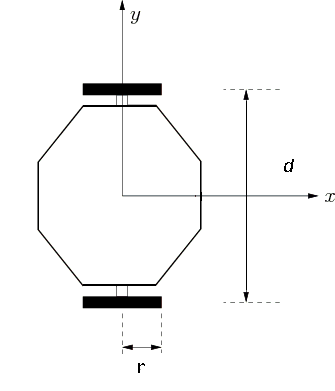
\includegraphics[width=0.5\columnwidth]{./ScoutAxis.png}
    \caption{Scout Axis}
    \label{fig:scout_axis}
\end{figure}
The control loop that we implemented looks as shown in figure \ref{fig:scout_loop}.
\begin{figure}[!h]
    \centering
    \includegraphics[width=\columnwidth]{./ControlLoopScout.png}
    \caption{Scout's Control Loop}
    \label{fig:scout_loop}
\end{figure}

\subsection{Decision Node: Probabilistic Model}
As it can be seen in figure \ref{fig:adele_structure} the Decision Node is the central block of this project and where its main focus should be. The role of the Decision Node in this project is to interpret the information coming from the Kinect Node and based on the results of the Training Set make a decision on the command that should be sent to the Action Node.

The Decision Node works together with a Training Set. This Training Set is a set of small videos where one user stands in front of the camera and behaves like if he were in a normal human-human interaction. Some examples of interactions are the following:
\begin{itemize}
\item User moves around; waves; goes towards the camera; hands an object
\item User waves; calls; gives an high-five
\item User calls; goes away
\end{itemize}
For saving the information in the Training Set, the following structure is used:\\

$\big[Distance, [Gesture, Timestamp, Velocity_x]_1,...$\\$
[Gesture, Timestamp, Velocity_x]_5\big]$

To every structure arriving the Training Set, a label is given. This label represents the action that Adele should take as a response to that particular human behaviour.

To explain the idea behind this labelling let's use the waving gesture as an example. The moment immediately before the user starts waving, the information coming from the Kinect is already labelled as a "Waving", so that Adele knows that when the user is at that particular distance and moves his arm at that particular velocity and with that amplitude of movement, he is waving at her and she must react properly (waving back). Ideally the features read by the Kinect node are sufficient to distinguish the "waving" from any other gesture and therefore Adele starts reacting before she sees the complete movement.

As mentioned before, the labels that were given, depend only on the person's movement/gesture and represent Adele's reaction. Table \color{red}\ref{tab:expected_response} \color{black} shows the dependencies between both aspects.
\begin{table}[!h]
\centering
\label{tab:expected_response}
\begin{tabular}{|c|c|}
\hline
\textbf{Person's gesture/movement} & \textbf{Adele's response} \\ \hline
Waving                           & Wave                                 \\
Handing an object                & Grab                            		\\
Calling                          & Go meet user                         \\
Go away                          & Return to home                       \\
High-Five                        & Low-Five                             \\
Low-Five                         & High-Five                            \\
Random                           & NOP                                  \\ \hline
\end{tabular}
\caption{Expected response from Adele}
\end{table}

The next step in the implementation of the Decision Node concerns Adele's learning. The Training Set was divided into two parts, one containing 80\% and the other with the remaining 20\%, the latter being called the validation set.

Regarding how the validation is done, there were some different machine learning algorithms that were tested, such as: SVM, Linear SVM, Logistic Regression, 3 Nearest Neighbours, AdaBoost and Stochastic Gradient Descent. The algorithm that presented the best performance using 10-fold cross-validation was the SVM and therefore that was the chosen one.

\color{red}
.......preciso de uma ajudinha para perceber exactamente o hip hop dos acrescimos de probabilidades e do threshold.....
\color{black}

\begin{table}[]
\centering
\begin{tabular}{cccccccc}
Previous|Next                        & \textbf{NOP} & \textbf{Wave} & \textbf{H5} & \textbf{L5} & \textbf{Go} & \textbf{Grab} & \textbf{Return} \\ \cline{2-8} 
\multicolumn{1}{c|}{\textbf{NOP}}    & 1/7          & 1/7           & 1/7         & 1/14        & 1/7         & 3/14          & 1/7             \\
\multicolumn{1}{c|}{\textbf{Wave}}   & 1/7          & 0             & 0           & 1/7         & 3/7         & 2/7           & 0               \\
\multicolumn{1}{c|}{\textbf{H5}}     & 1/6          & 1/6           & 0           & 1/6         & 1/6         & 1/6           & 1/6             \\
\multicolumn{1}{c|}{\textbf{L5}}     & 2/7          & 0             & 0           & 0           & 0           & 2/7           & 3/7             \\
\multicolumn{1}{c|}{\textbf{Go}}     & 1/14         & 0             & 1/7         & 1/7         & 0           & 3/7           & 3/14            \\
\multicolumn{1}{c|}{\textbf{Grab}}   & 2/7          & 0             & 1/7         & 1/7         & 0           & 0             & 3/7             \\
\multicolumn{1}{c|}{\textbf{Return}} & 1/6          & 1/6           & 1/6         & 1/6         & 1/6         & 1/6           & 0              
\end{tabular}
\caption{My caption}
\label{my-label}
\end{table}
